\chapter*{Appendix F}\label{AppendixF}
\vspace{-1.75cm}
\subsection{Gaussian process priors}

Preliminary results from analysis with Gaussian process smoothness priors. The estimates
for bias toward the majority party are slightly different (and less stable) than the estimates 
from the model with $RW_1$ priors, but both suggest similar trends in bias over time.  
We are currently studying the sensitivity of the results to the chosen kernel (covariance function).  
The plot below is generated using a generalized squared exponential kernel.  

\begin{figure}[h]
\centering
	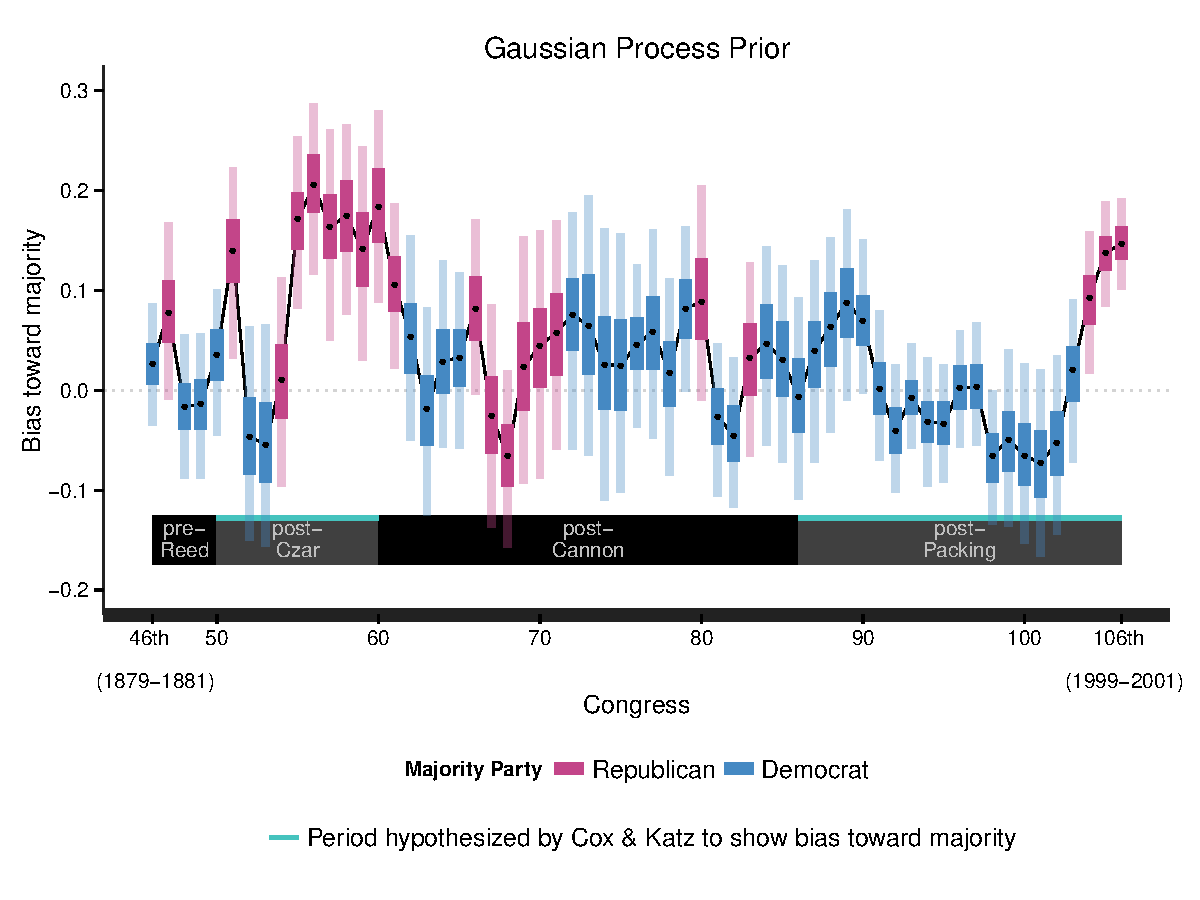
\includegraphics[scale=0.7]{sections/figs/ck_replication_gp}
\caption*{Vertical bars are 50\% and 95\% intervals. Points are posterior medians.}
\label{fig:gp_prior}
\end{figure}


